\chapter{Chemistry on a Computer}
\label{chapter:theory}
\section{Quantum Mechanics and Chemistry}\label{section: QM}
\subsection{Overview}\label{section: QM_overview}
The development of quantum mechanics in the early 20th century armed scientists with the tools to calculate the microscopic properties of matter. In chemistry, the postulates of quantum mechanics can be applied to calculate relative energies of molecules, molecular geometries, ratios of products of chemical reactions, transition states, spectra, and any other phenomenon of interest. However, whilst in principle any property can be calculated exactly by the \schro{} equation, the analytical solution is only obtainable for systems with one electron. For systems larger than this, and therefore anything of observable chemical relevance, the computational expense on even modern computer architecture is intractable. 

To overcome this, a number of approximations are used in the field of computational chemistry to solve the multielectron problem. In general, as the number of atoms one wants to model increases, qualitative nature of the result also increases. Computational chemistry methods can generally be split into the types of approximations made and the number of atoms the method wishes to treat. In biophysical process and the modelling of proteins on the scale of tens of thousands of atoms, quantum mechanics is ignored completely. Forcefields are used to calculate the energy corresponding to a set of atomic coordinates in what are known as the \ac{MM} class of methods. The interactions between atoms are defined by analytical potentials, such as for bond stretches, bends, and angles, and are parameterised for different types of molecules using more accurate methods. This procedure is time-consuming and makes the forcefield specific to the systems it was fitted to, but enables computationally facile access to molecular geometries and properties of large systems.

At the other end of the scale the electronic structure is included through wavefunction or \ac{DFT} techniques. For the applications involved in this thesis, involving photoinduced phenomena, the activity of the electrons is paramount, and as such it is these methods which are utilised herein. In the next sections, the importance of the \schro{} equation shall be established, which along with the Born-Oppenheimer approximation enables the calculation of electronic properties through the simplest wavefunction method, the \ac{HF} method. Methods to improve the \ac{HF} approximation are then introduced, followed by the paradigm shift offered by \ac{DFT}. The first two sections of this Chapter focus on methods to obtain ground state properties, whilst in Section \ref{section: Photo} excited state methods shall be discussed. 
%%%%%%%%%%%%%%
%%%%%%%%%%%%%%
\subsection{The \schro{} Equation}\label{section: QM_schrodinger}
%%%%%%%%%%%%%%
%%%%%%%%%%%%%%
The wavefunction $\Psi$ contains all the information about the quantum state of the system at a position and time. As Newton's second law ($\bm{\mathrm{F}}=m\bm{\mathrm{a}}$) gives a classical particle's position and moment at each time period, thus describing it's classical state, so the time-dependent \schro{} equation does for wavefunction, and has the general form
\begin{equation}\label{equation: td-schro}
    i\hbar{}\frac{\partial \Psi(\bm{R},\bm{r},t)}{\partial t}=\hat{H}\Psi(\bm{R},\bm{r},t)
\end{equation}
where $\hbar=\frac{h}{2\pi}$ and $\hat{H}$ is the Hamiltonian operator for electrons at $\bm{r}$ and nuclei at $\bm{R}$. Separating the spatial part from the temporal part yields the time-dependent version of the \schro{} equation, which using the bra-ket notation of Dirac is\cite{Schrodinger1926}
\begin{equation}\label{equation: ti-schro}
   \hat{H}\ket{\Psi}=E\ket{\Psi}.
\end{equation}
This is an eigenvalue equation, where the Hamiltonian operator acts on the wavefunction to give the energy $E$ of the system. For a system of $N$ electrons and $M$ nuclei, the Hamiltonian calculates the kinetic ($T$) and potential ($V$) energy contributions of the electrons and nuclie towards the total energy of the system,
\begin{equation}\label{equation: H-simple}
\hat{H}=\hat{T}_{e}+\hat{T}_{n}+\hat{V}_{n-e}+\hat{V}_{e-e}+\hat{V}_{n-n}
\end{equation}
\begin{equation}\label{equation: H}
   \hat{H}=\underbrace{-\sum_{i=1}^{N}\frac{1}{2}\nabla_{i}^2 - \sum_{A=1}^{M}\frac{1}{2M_{A}}\nabla_{A}^2}_\text{kinetic terms}-\underbrace{\sum_{i=1}^{N}\sum_{A=1}^{M}\frac{Z_{A}}{r_{iA}}+\sum_{i=1}^{N}\sum_{j>{i}}^{N}\frac{1}{r_{ij}}+\sum_{A=1}^{M}\sum_{B>{A}}^{M}\frac{Z_{A}Z_{B}}{R_{AB}}}_\text{electrostatic terms}
\end{equation}
where $i$ and $j$ are electrons and $A$ and $B$ are nuclei. The first two terms are the operators for the kinetic energy of the electrons and the nuclei, where the Laplacian operator $\nabla^{2}$ is the second derivative of position. The next three terms are the electrostatic operators, summing the Coulomb interactions in the system;  the attractive interaction between electrons and the nuclei (of charge $Z$); the repulsive interaction between electrons; and the repulsive interaction between nuclei. Atomic units are used throughout, such that the electronic charge and mass are neglected. The $R$ and $r$ terms in the electrostatic parts denote the distance between nuclei and electrons.
%To calculate the energy $E$ , however, an eigenfunction for Equation \ref{equation: ti-schro}is required, corresponding to a wavefunction describing the electronic state.\cite{aszabo82:qchem}

In the hydrogen atom, the $\hat{V}_{e-e}$ and $\hat{V}_{n-n}$ can be neglected since there is only one proton and one electron, and the exact solution for the energy can be calculated since the wavefunction can be constructed analytically. However, for larger systems with many electrons and nuclei, Equation \ref{equation: ti-schro} cannot be solved. As such, a number of approximations must be made. The most fundamental of these is Born-Oppenheimer approximation.
%%%%%%%%%%%%%%
%%%%%%%%%%%%%%
\subsection{The Born-Oppenheimer Approximation}\label{section: QM_bornoppenheimer}
%%%%%%%%%%%%%%
%%%%%%%%%%%%%%
Separation of variables is a key concept in quantum chemistry, where a complex problem is broken down into constituent parts. This method is used to simplify the solving of Equation \ref{equation: ti-schro} by separating the electronic terms from the nuclear terms, and is known as the Born-Oppenheimer Approximation\cite{Born1927}
\begin{equation}
    \Psi_{BO}(\bm{R},\bm{r})=\Theta_{\bm{R},\bm{r}}\Phi_{\bm{r}}.
\end{equation}
where $\Theta_{\bm{R},\bm{r}}$ is the nuclear wavefuction and $\Phi_{\bm{r}}$ is the electronic wavefunction. The separation of terms is rooted in the fact that the nuclei are vastly heavier than electrons, and so it can be approximated that the nuclei are static with respect to the electrons. Equation \ref{equation: ti-schro} is solved, then, in two steps. First, the electronic structure is solved with ``clamped" nuclei, resulting in an electronic energy which is a parametric function of the nuclear coordinates. By concentrating on just the electronic terms, the \textit{electronic} Hamiltonian $\hat{H}_{e}$ becomes
\begin{equation}\label{equation: Hel}
     \hat{H}_{e}=\underbrace{-\sum_{i=1}^{N}\frac{1}{2}\nabla_{i}^2}_\text{kinetic term}-\underbrace{\sum_{i=1}^{N}\sum_{A=1}^{M}\frac{Z_{A}}{r_{iA}}+\sum_{i=1}^{N}\sum_{j>{i}}^{N}\frac{1}{r_{ij}}}_\text{electrostatic terms}.
\end{equation}
and the electronic \schro{} equation is then
\begin{equation}\label{equation: ti-schro-el}
   \hat{H}_{e}\ket{\Phi}=E_{e}\ket{\Phi}
\end{equation}

The total wavefunction $\Psi$ can considering multiple electronic states can be constructed from the combination of the electronic functions for each state $I$ and the corresponding nuclear wavefunction $\Theta_{I}$ in what is known as the Born-Huang expansion\cite{Born1954}
\begin{equation}
    \Psi(\bm{R},\bm{r})=\sum_{I}\Theta_{I}\Phi_{I}.
\end{equation}

When the nuclei are stationary, their kinetic energy is zero and the complete Hamliltonian is just the electronic Hamiltonian. For vibrating molecules, Equation \ref{equation: ti-schro-el} is solved at the required nuclear configuration, for electronic state $I$, and the time-evolution of the nuclear wavefunctions is\cite{Worth2004}
\begin{equation}\label{equation: nucwavefunctions}
    i\hbar{}\frac{\partial{}\Theta_{I}}{\partial{}t}=[\hat{T_{n}}+E_{I}]\Theta_{I}\underbrace{-\sum_{I}\hat{\Lambda}_{JI}\Theta_{I}}_\text{Nonadiabtic couplings}
\end{equation} 
%%%%%%%%%%%%COMMENT
\begin{comment}
\begin{equation}
    \sum_{A}\frac{1}{2M_{A}}\sum_{J\neq{}I}\hat{\Lambda}_{JI}\Theta_{I}=[\hat{T_{n}}+E_{I}(\bm{R})-E]\Theta_{I}
\end{equation} 
\end{comment}
%%%%%%%%%%%%COMMENT
where the energy of $E_{I}$ is the expectation value of the electronic Hamiltonian ($\bra{\Phi_{I}}\hat{H_e}\ket{\Phi_{I}}$). The highlighted \textit{nonadiabtic coupling} operator $\hat{\Lambda}_{JI}$ couples electronic state $I$ with electronic state $J$. In the adiabatic Born-Oppenheimer approximation, this coupling is completely neglected and the time-evolution of the nuclei becomes\cite{Yonehara2012}
\begin{equation}\label{equation: BO}
    i\hbar{}\frac{\partial{}\Theta_{I}}{\partial{}t}=[\hat{T_{n}}+E_{I}]\Theta_{I}
\end{equation} 
The nuclear motion is thus determined by the electronic energy of uncoupled \textit{adiabatic} states, and the nuclei move on the \ac{PES} of state $I$. $\hat{\Lambda}_{JI}$ contains the \textit{nonadiabatic} couplings, which become important when electronic states converge in energy. This shall be discussed in Section \ref{section: photo_conicals}

The Born-Oppenheimer approximation helps divide the problem into electronic and nuclear parts. However, solving the electronic problem exactly for many electron systems is impossible. In the next section, the mathematical building blocks of electronic structure methods, basis sets, shall be briefly described, after which methods to solve the electronic problem are introduced, starting with the \acf{HF} method. The \ac{HF} method is the fundamental quantum chemical approach to solve the many electron problem.
%%%%%%%%%%%%%%
%%%%%%%%%%%%%%
\subsection{Basis Sets}\label{section: methods_basisets}
%%%%%%%%%%%%%%
%%%%%%%%%%%%%%
Molecular orbitals are constructed from the linear combination of atomic orbitals. These atomic orbitals are represented by mathematical functions called a basis set. A complete set these functions, without any other approximations, would lead to the computation of the exact wavefunction (or energy). However, since an infinite basis set is not possible, another source of error in the electronic structure arises from the truncation of the basis set and the number of functions used. Atom-centred basis sets typically consist of Gaussian functions, which hold many numerical advantages over other functional forms for the wavefunction. To adequately describe valence orbitals, more than one basis function is used in what is known as the split valence. Adding polarisation and diffuse functions aid the long range description of the atomic orbital.\cite{Cramer2002}

For solid state calculations involving periodic systems, it is computationally more efficient to switch from atomic centred orbitals to periodic functions. In the solid state community, planewave basis sets are used to sample the unit cell, where the wavefunction is described by one-electron periodic functions ($e^{ikr}$). The wavefunction is constructed by summing these planewaves up to an energy cut-off as a function of the frequency. Often the core electrons are approximated by pseudopotentials to lower the computational cost of computing high frequency planewaves.\cite{Young2001} 

In the work presented in this thesis, almost all calculations involve atom-centred basis sets. Periodic DFT using planewaves are used to optimise the unit cells of molecular crystals, from which clusters are extracted and energies calculated as described in Section \ref{section: excited_states_crystals}. 

%%%%%%%%%%%%%%
%%%%%%%%%%%%%%
\section{Quantum Chemical Methods}\label{section: methods}
\subsection{The Hartee-Fock Method}\label{section: methods_HF}
%%%%%%%%%%%%%%
%%%%%%%%%%%%%%
In the \ac{HF} method, a single electron in an $N$-electron system moves within the field produced by the nuclei and the other $N$-1 electrons.\cite{hartree_1928} The intractable $N$-electron wavefunction $\Phi$ is simplified to be a product of $N$, one-electron wavefunctions $\chi$,
\begin{equation}
\ket{\Phi}=\ket{\chi_{1}\chi_{2}...\chi_{i}..\chi_{N}}.
\end{equation}
where $\chi$ are spin orbitals of each electron in the system. The spin orbitals consist of a spatial functional and a spin function, an infinite number of which could provide an exact solution. However, in practical terms a basis set of atomic functions is supplied, as described in Section \ref{section: methods_basisets}.\cite{szabo1996}
 
 From the Pauli exclusion principle, no two electrons may share exactly the same four quantum numbers (i.e occupy the same spatial and spin orbital). Since electrons are fermions, the electronic wavefunction is \textit{antisymmetric}, meaning that a change in the orbital must result in the wavefunction changing sign. This is enforced using Slater Determinants.\cite{Slater1929} This is most easily seen for a two-electron system for electrons at positions $\bm{x}_{1}$ and $\bm{x}_{2}$, where orbital $\chi_{1}$ contains electron at $\bm{x}_1$ and orbital $\chi_{2}$ contains electron at $\bm{x}_2$, with a normalisation factor of $N^{-\frac{1}{2}}$
\begin{equation}
\begin{split}
\Phi(\bm{x}_{1},\bm{x}_{2})&=\frac{1}{\sqrt{2}}\{\chi_{1}(\bm{x}_{1})\chi_{2}(\bm{x}_{2})-\chi_{1}(\bm{x}_{2})\chi_{2}(\bm{x}_{1})\}\\
&=\frac{1}{\sqrt{2}}
\begin{vmatrix}
\chi_{1}(\bm{x}_{1})&\chi_{2}(\bm{x}_{1})\\
\chi_{1}(\bm{x}_{2})&\chi_{2}(\bm{x}_{2})
\end{vmatrix}
\end{split}
\end{equation}
where by taking the determinant, the antisymmetry is ensured since exchanging the electrons changes the sign of the determinant. In the determinant, the rows consist of the electrons while the columns contain the orbitals. In the \ac{HF} method, the wavefunction is approximated by a single Slater Determinant, and therefore \ac{HF} is known as a single-determinant, or single-reference, method.  As well as ensuring antisymmetry, the Slater determinant wavefunction also introduces exact exchange (or HF exchange), a quantum mechanical property for electrons of parallel spin.\cite{szabo1996}

The variational principle states that the true ground state wavefunction will always be less than or equal to a trial wavefunction, meaning that the guessed spin orbitals will never undershoot the true energy. As such, 
\ac{HF} is a purely iterative method where the energy is computed for a set of trial spin orbitals, the spin orbitals are altered, and the energy is guessed again. This is repeated until convergence. 

To calculate the ``best" set of orbitals, the interactions in the electronic Hamiltonian are split into one-electron and two electron terms. The one electron terms are collected by the core Hamiltonian operator $\hat{h}_{i}$, involving the kinetic energy of the electrons and the electron-nuclei interactions,
\begin{equation}
    \hat{h}_{i}=-\frac{1}{2}\nabla_{i}^{2}-\sum_{A=1}^{M}\frac{Z_{A}}{r_{iA}}.
\end{equation}
The antisymmetric nature of the Slater determinent results in two operators for the electron-electron interaction, a Coulomb operator $\hat{J}_{ij}$ and an exchange operator $K_{ij}$, which act on orbital $\chi_{i}$ to determine the effect of the remaining orbitals,
\begin{equation}
    \hat{J}_{ij}\chi_{i}=\chi_{i}\int{\frac{\chi^{\ast}_{j}\chi_{j}}{r_{ij}}d\bm{x}_{2}}
\end{equation}
\begin{equation}
    \hat{K}_{ij}\chi_{i}=\chi_{j}\int{\frac{\chi^{\ast}_{j}\chi_{i}}{r_{ij}}d\bm{x}_{2}}.
\end{equation}
The Coulomb operator determines the Coulomb potential felt by electron $i$ in orbital $\chi_{i}$ from electron $j$ in orbital $\chi_{j}$. This is done by \textit{averaging} the interaction over all of the spatial coordinates of electron $j$. As such, $J_{ij}$ represents the average, or \textit{mean-field}, local potential felt by electron $i$. For this reason, the \ac{HF} method is often called a mean-field approach. The exchange operator $K_{ij}$ is a result of the antisymmetric Slater determinant, and is a quantum mechanical artefact of the fact that electrons are by nature  indistinguishable, and the exact labelling ($i$,$j$) has no physical meaning.\cite{szabo1996}

The one-electron and two-electron operators are collected by the Fock operator $\hat{F}$, such that
\begin{equation}
    \hat{F}=\hat{h}_{i}+\sum_{j\neq{}i}^{\frac{N}{2}}{[\hat{J_{ij}}-\hat{K_{ij}}]}
\end{equation}
The two electron terms run over only half of the electrons ($\frac{N}{2}$) to ensure interactions are not double counted, while the condition of $j\neq{}i$ means that an electron cannot interact with itself. 

The Fock operator allows Equation \ref{equation: ti-schro} to be solved in the \ac{HF} method through,
\begin{equation}\label{equation: Fock-operator}
    \hat{F}\ket{\Phi}=E\ket{\Phi}
\end{equation}
an eigenvalue equation solved by altering the orbitals until energy convergence is reached. In practice, for a closed shell system, the molecular orbital $\chi_{i}$ consists of a linear combination of $K$ atomic basis functions,
\begin{equation}\label{equation: expansion}
    \chi_{i}=\sum_{\mu=1}^{K}C_{ui}\phi_{\mu}\qquad\quad{}i=1,2,..,K
\end{equation}
The Roothaan-Hall equations are then used to solve Equation \ref{equation: Fock-operator} in matrix form,\cite{Roothaan1951,Hall1951}
\begin{equation}
    \bm{FC}={\bm{SC\epsilon}}
\end{equation}
where $\bm{F}$ is the Fock matrix containing the elements from the Fock operator, $\bm{C}$ contains the expansion coefficients from Equation \ref{equation: expansion} and $\bm{S}$ is the overlap matrix containing the overlaps of atomic orbitals ($\bra{\phi_{i}}\ket{\phi_{j}}$). By diagonalising the Fock matrix, $\epsilon$ is a diagonal matrix containing the orbital energies. \ac{HF} is commonly named the \ac{SCF} approximation, since the Roothaan equations are solved until self-consistency is reached.


The \ac{HF} method is a powerful approach to solving the electronic part of the \schro{} equation. However, it has several severe drawbacks which hinder its application and have resulted in more sophisticated methods being developed to address the shortcomings within. The most serious of these for ground state, closed-shell systems is the correlation problem. While electrons of parallel spin have the required exchange correlation, the Coulomb correlation is completely neglected since each electron sees only an average field of the other electrons. In reality, the motion of one electron is dependent on the motion of each of the other electrons, as depicted in Figure \ref{figure: mean-field}. This results in the energy of the system in \ac{HF} being overestimated in respect to the true energy. A number of methods to overcome the lack of correlation have been developed, which use the \ac{HF} method as a starting point before calculating the electron correlation. These are called post-Hartree-Fock methods, and those most relevant to the work in this thesis are discussed in the next section.
\begin{figure}[t]
\centering
  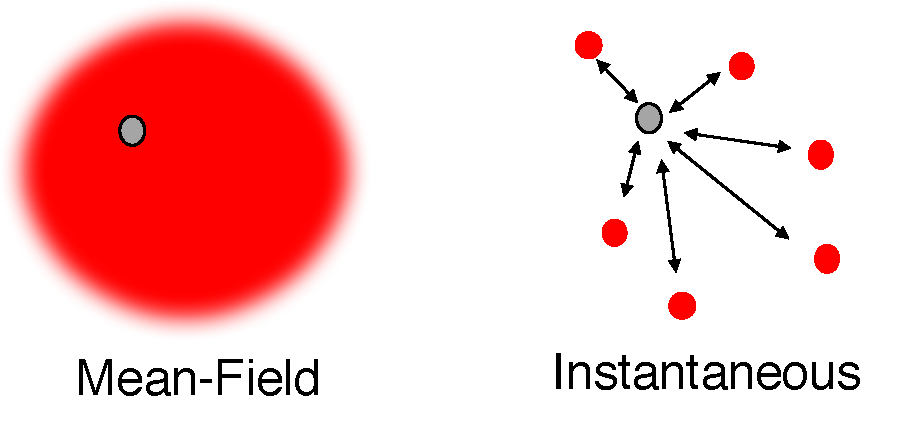
\includegraphics[width=0.4\linewidth]{2Theory/Mean_Field.pdf}
  \caption[Schematic of the mean-field approximation]{Depiction of the mean field electron interaction, where the electron of interest interacts with an average potential, rather than individually with each other electron.}
  \label{figure: mean-field}
\end{figure}

\subsection{Post-Hartre-Fock Methods}\label{section: methods_postHF}
%%%%%%%%%%%%%%
%%%%%%%%%%%%%%
\subsubsection{M{\o}ller-Plesset Perturbation Theory}
%%%%%%%%%%%%%%
Electron correlation energy can be added to the \ac{HF} energy by way of an external perturbative correction. In perturbation theory, the total Hamiltonian is divided into the zeroth-order part $\hat{H}_{0}$, which is the \ac{HF} Hamiltonian, and a perturbation $\hat{V}$, such that the eigenvalue equation becomes
\begin{equation}\label{equation: PT}
    \hat{H}\ket{\Phi_{i}}=(\hat{H}_{0}+\hat{V})\ket{\Phi_{i}}=\epsilon_{i}\ket{\Phi_{i}}.
\end{equation}
The eigenvalues and eigenfunctions of $\hat{H}_{0}$ are varied so that they become closer to the total Hamiltonian $\hat{H}$, which would then contain electronic correlation. This is done by the ordering factor $\lambda$, such that
\begin{equation}
    \hat{H}=\hat{H}_{0}+\lambda\hat{V}
\end{equation}
The true eigenvalues and eigenfunctions are expanded in a Taylor series in $\lambda$ up to $n$th order,
\begin{equation}\label{equation: MP2_energies}
    \epsilon_{i}=E_{i}^{(0)}+\lambda{}E_{i}^{(1)}+\lambda^{2}E_{i}^{(2)}+\lambda^{3}E_{i}^{(3)}+..+\lambda^{n}E_{i}^{(n)}
\end{equation}
\begin{equation}\label{equation: MP2_functions}
    \ket{\Phi_{i}}=\ket{\Phi_{i}^{(0)}}+\lambda{}\ket{\Phi_{i}^{(1)}}+\lambda^{2}\ket{\Phi_{i}^{(2)}}+\lambda^{3}\ket{\Phi_{i}^{(3)}}+..+\lambda^{n}\ket{\Phi_{i}^{(n)}}
\end{equation}
After inserting Equations \ref{equation: MP2_energies} and \ref{equation: MP2_functions} into Equation \ref{equation: PT} and collecting terms by order, the general expression for the total energy is
\begin{equation}
E_{i}=E_{i}^{(0)}+\sum_{n=1}^{n}\bra{\Phi_{i}^{(0)}}\hat{V}\ket{\Phi_{i}^{(n-1)}}
\end{equation}
The perturbation operator $\hat{V}$ introduces the Coulomb repulsion between electrons, which when combined with excited Slater determinants, recovers the \textit{dynamic} correlation energy. In most chemical applications, the method is contracted at second-order, and was initially employed by C. M{\o}ller and M.S. Plesset to obtain the correlation energy, hence the acronym \ac{MP2} is often used.\cite{Moller1934} Since MP is perturbative, the MP-calculated energy can be lower than the true energy, making it a non-variational method.
%%%%%%%%%%%%%%
\subsubsection{Coupled Cluster Theories}
%%%%%%%%%%%%%%
In an alternative approach to perturbation theory, \ac{CC} methods were introduced in the 1960s to account for electron correlation.\cite{Cizek1966,Paldus1972} \ac{CC} theory uses excited determinants by means of a Taylor expansion with an exponential operator
\begin{equation}\label{equation: cc}
    \ket{\Phi_{CC}}=e^{\hat{T}}\ket{\Phi_{0}}
\end{equation}
where $\ket{\Phi_{0}}$ is the \ac{HF} wavefunction and $\hat{T}$ is the cluster operator. The cluster operator produces a sum of excitation operators up to the truncation level $n$
\begin{equation}\label{equation: T}
    \hat{T}=\hat{T}^{(1)}+\hat{T}^{(2)}+\hat{T}^{(3)}+...+\hat{T}^{(n)}
\end{equation}
where $n$ is the excitation number. $\hat{T}^{(1)}$ includes all single excitations and $\hat{T}^{(2)}$ includes all double excitations, \textit{etc}.
%%%%%%%%%%%%%
%%%%%%%%%%%%
%For the first order, the contribution of all single excited determinants is 
%\begin{equation}
%    \hat{T}^{(1)}\ket{\Phi_{0}}=\sum_{i}^{occ}\sum_{a}^{vir}t_{i}^{a}\phi_{i}^{a}
%\end{equation}
%where $\phi_{i}^{a}$ is the excitation of an electron from occupied orbital $\phi_{i}$ to virtual orbital $\phi_{a}$, and $t_{i}^{a}$ is the amplitude given to this excitation.
%%%%%%%%%%%%%
%%%%%%%%%%%%
Substituting \ref{equation: T} into \ref{equation: cc}, and truncating at $n=2$, yields the coupled cluster wavefunction
\begin{equation}\label{equation: CCwavefunctioncomplete}
\ket{\Phi_{CC}}=e^{\hat{T}}\ket{\Phi_{0}}=\big[1+\hat{T}^{(1)}+(\hat{T}^{(2)}+\frac{\hat{T}^{2(1)}}{2})\big]\Phi_{0}
\end{equation}
As for perturbation theory, \ac{CC} theory is usually referred to by the trunctation level, for example CCSD refers to coupled cluster with single and double excitations. CCSD scales at $N^{6}$, adding considerable expense to the \ac{HF} method, which scales at $N^{4}$ (where $N$ is the number of basis functions).

%%%%%%%%%%%%%%
\subsection{Multireference Methods}\label{section: methods_multiconf}
%%%%%%%%%%%%%%
The methods described so far use \ac{HF} as a starting point and are thus built on a single-reference wavefunction. For a closed-shell system of an even number of electrons, orbitals are all doubly occupied. However, in many chemical processes, the electronic structure will deviate from this description and the wavefunction will not be dominated by one single electronic configuration, for example in bond dissociation, excited state processes, or when metallic elements are introduced. To describe these scenarios, the ground state wavefunction must incorporate other relevant electronic configurations, where more than one Slater determinant is used in the ground state wavefunction. These are termed multireference or multiconfigurational methods, and the multireference wavefunction is expressed as
\begin{equation}
    \ket{\Psi}=\sum_{m}c_{m}\ket{m}
\end{equation}
where $\ket{m}$ is the configuration state function containing optimised molecular orbitals and $c_{m}$ is the expansion coefficient for the state. In multireference methods, the molecular orbitals are divided into subspaces, where the active space contains the orbitals from which the important configurations are taken. In the configuration interaction method, the active space contains all of the molecular orbitals, with all excitations between the orbitals are considered, and thus all possible configurations are used in the wavefunction. This recovers the exact wavefunction (with an infinite basis set), but is prohibitively expensive such is the vast number of possible determinants, although these can be truncated to include only single excited states. More common is to use an active space containing occupied and virtual orbitals selected for their relevance for the problem in hand, and to only include excitations from within the $m$ active orbitals for $n$  electrons. This is called the \ac{CAS} method, which when used in combination with \ac{HF} for the remaining core orbitals (outwith the active space), is denoted \ac{CASSCF}.\cite{Roos1980} Due to the factorial scaling with the number of active orbitals, further space decomposition methods have been introduced through \ac{RAS}, where only certain excitations are allowed. Furthermore, using a state-averaging procedure can optimize the configuration state-functions for multiple states, to describe regions of strong electronic mixing. With these methods, the key parameter is often the choice of the active space - which orbitals to include, how many of them, and how many corresponding electrons. This is not a black-box procedure and will vary depending on the system of interest, the phenomena being modelled, and the computational resources available.\cite{Lischka2018} Recently, algorithms for automatic active-space selection procedures have been proposed.\cite{Stein2016,Bao2018}

Electron correlation can be divided into dynamic and static contributions. By incorporating the multireference character of the wavefunction, \textit{static} correlation is recovered in solving the \schro{} equation. The dynamical part is added on top of a reference wavefunction in the form of excitations, typically through perturbation theory as discussed in \ref{section: methods_postHF}. As such, most of the total correlation can be recovered by combining a multireference wavefunction with perturbation theory. This can produce accurate ground and excited state properties for chemical systems, although with rather large computational expense.\cite{Ramos-Cordoba2017,Stein2016a} A favoured approach is to combine \ac{CAS}\ac{SCF} with a \ac{PT2} calculation (\ac{CAS}\ac{PT2}), providing an effective protocol to calculate excited states. 
\subsection{Density Functional Theory}\label{section: theory_dft}
%%%%%%%%%%%%%%
The methods introduced thus far access chemical properties through some approximation of the wavefunction. An alternative approach is to disregard the wavefunction altogether and instead use the electron density to calculate microscopic properties of matter. This replaces the 3$N$ (+spin) variable of wavefunction methods by just 3 (+spin) spatial variables, allowing significant speed-up in \ac{DFT}. In 1964, Pierre Hohenberg and Walter Kohn proved a unique 1:1 correspondence exists between the ground state energy and the ground state density, and that all ground properties of a given $N$-electron system can be calculated from the ground state electron density ($\rho$).\cite{Kohn1964} The energy is thus a \textit{functional} (function of a function) of the electron density produced by a wavefunction,
\begin{equation}
    E[\rho]=\bra{\Psi[\rho]}\hat{T}+\hat{V}\ket{\Psi[\rho]}
\end{equation}
and, like \ac{HF}, obeys the variational principle.

\ac{DFT} is a mathematically exact formulation. However, the exact form of the functional relating the density to the energy is unknown. In 1965, Kohn and Sham developed a self-consistent approach to attain an approximation of the energy functional in equations that are ``analogous to the conventional Hartree and Hartree-Fock equations, and, although they also include correlation effects, they are no more difficult to solve."\cite{Kohn1965} In the Kohn-Sham system, a non-interacting system mimics the real interacting electron density. As in \ac{HF} where one-electron wavefunctions construct the N-electron wavefunction, so do single particle orbitals (Kohn-Sham orbitals $\phi$) construct the electron density,
\begin{equation}
    \rho=\sum_{j=1}^{N}|\psi_{j}|^{2}.
\end{equation}
The Kohn-Sham expression for the energy functional is written in terms of the kinetic and electrostatic interactions,
\begin{equation}
    E[\rho]=T_{e}[\rho]+E_{n-e}[\rho]+E_{e-e}[\rho].
\end{equation}
The most straightforward term to evaluate is the nuclear-electron interaction, which can be expressed as an electrostatic potential $V_{n}$ from the nuclei acting on the electronic density, 
\begin{equation}
    V_{n-e}[\rho]=\int{V_{n}(\bm{r})\rho(\bm{r})\mathrm{d}\bm{r}}.
\end{equation}
The electron-electron interaction can be separated into a classical, Coulomb-type expression and the quantum mechanical \ac{XC} part
\begin{equation}
    E_{e-e}[\rho]=\frac{1}{2}\underbrace{\int{}\frac{1}{r_{e_{1}e_{2}}}\rho(\bm{r}_{e_{1}})\rho(\bm{r}_{e_{2}})\mathrm{d}\bm{r}_{e_{1}}\mathrm{d}\bm{r}_{e_{2}}}_\text{Classical}+\underbrace{\vphantom{ \left(\frac{a^{0.3}}{b}\right) }E_{e-e}^{XC}[\rho]}_\text{XC}
\end{equation}
The kinetic energy of the interacting system is replaced by the kinetic energy of the non-interacting system, with the correction incorporated in to the \ac{XC} functional. It is the \ac{XC} functional which contains the crux of the problem in \ac{DFT}, since the exact form is unknown. It must be approximated. Much of \ac{DFT} development is focused on developing more accurate functionals to better describe specific chemical problems.

The first approximation to the functional is the \ac{LDA}. The LDA was originally proposed by Kohn and Sham in 1965 and depends only on the density at the coordinate in question. LDA approximates the molecular \ac{XC} energy by the \ac{XC} energy of a uniform electron gas. The \ac{XC} energy at a point in the molecule is then compared to a homogeneous electron gas with that density, for which the exchange can be solved analytically and the correlation is approximated through, for example, Monte-Carlo simulation.\cite{Ullrich2012} LDA works surprisingly well in structure prediction, given that the UEG has a uniform density whereas in reality the density varies with position in molecular systems. To incorporate the change of electron density with position, the \ac{GGA} functions include the density gradient, offering improved total energies, energy barriers, and geometries. Of the \ac{GGA} functionals, the PBE functional has become one of the most used in quantum chemistry.\cite{Perdew1996}

Hybrid functionals improve upon the \ac{GGA}s by including a percentage of \ac{HF} exchange energy. The \ac{XC} energy is expressed as a combination of the \ac{DFT} derived \ac{XC} and the \ac{HF} exchange energy. The hybrid version of PBE, PBE0, incorporates exact exchange \textit{via}
\begin{equation}
    E_{XC}^{PBE0}=\alpha{}E_{X}^{HF}+(1-\alpha{})E_{X}^{PBE}+E_{C}^{PBE}.
\end{equation}


One of the key errors in Kohn-Sham \ac{DFT}, using the types of functionals introduced thus far, is the self-interaction error. In \ac{HF}, the electron-electron interaction of the Hamiltonian ensures that an electron will interact with all the other electrons in the system but itself. In \ac{DFT}, each electron interacts with the entire electron density and thus with itself. If 100\% exact exchange is used this error is exactly cancelled. However, since this is not present in \ac{LDA}s or \ac{GGA}s, the \ac{XC}-potential does not show the correct asymptotic behaviour, and is only partially remedied by the small percentage of \ac{HF} exchange in hybrids. At large interelectronic distances, the self-interaction results in incorrect long-range asymptotic behaviour, where the \ac{XC} potential falls off more rapidly than 1/$R$.

To remedy this, a class of functionals called \acp{RSH} has been developed. The exchange is split into short- and long-range parts, where the short-range exchange will typically be represented by a local or semi-local functional, while the long range exchange is treated by \ac{HF} exchange. The distance at which the behaviour changes is determined by the range-separation parameter. Therefore, the long-range behaviour can be corrected due to having exact exchange. Whilst hybrid functionals are the most widely used in present day computational chemistry, it is certainly not a ``one size fits all" situation, since different functionals are developed to meet certain requirements, with development being ``property-driven" as much as rooted in theory. In particular, for dealing with excited states in \ac{TDDFT}, hybrid functionals have known and systamic failings, which the \ac{RSH} functionals aim to address. This shall be discussed in the next section, where the theory and techniques for modelling excited states are introduced.
%%%%%%%%%%%%%%%%%%%%%%%%%
%%%%%%%%%%%%%%%%%%%%%%%%%
\section{Modelling Electronically Excited States}\label{section: Photo}
%%%%%%%%%%%%%%%%%%%%%%%%%
%%%%%%%%%%%%%%%%%%%%%%%%%
\subsection{Overview}\label{section: photo_overview}
Thus far the methods introduced generally address thermal chemical processes, i.e those which occur in the electronic ground state. Modelling electronically excited states is a considerably more complex task, in terms of both the number of possible reaction paths and the methods needed to describe them. Some of these are illustrated in Figure \ref{figure: Jablonski}. The \acf{PES}, briefly introduced in Section \ref{section: QM_bornoppenheimer}, is absolutely central in understanding excited-state processes. It is through probing the \ac{PES} that feasible pathways, and thus chemical mechanisms, are elucidated and physical observables are rationalised theoretically.

\begin{figure}[t]
\centering
  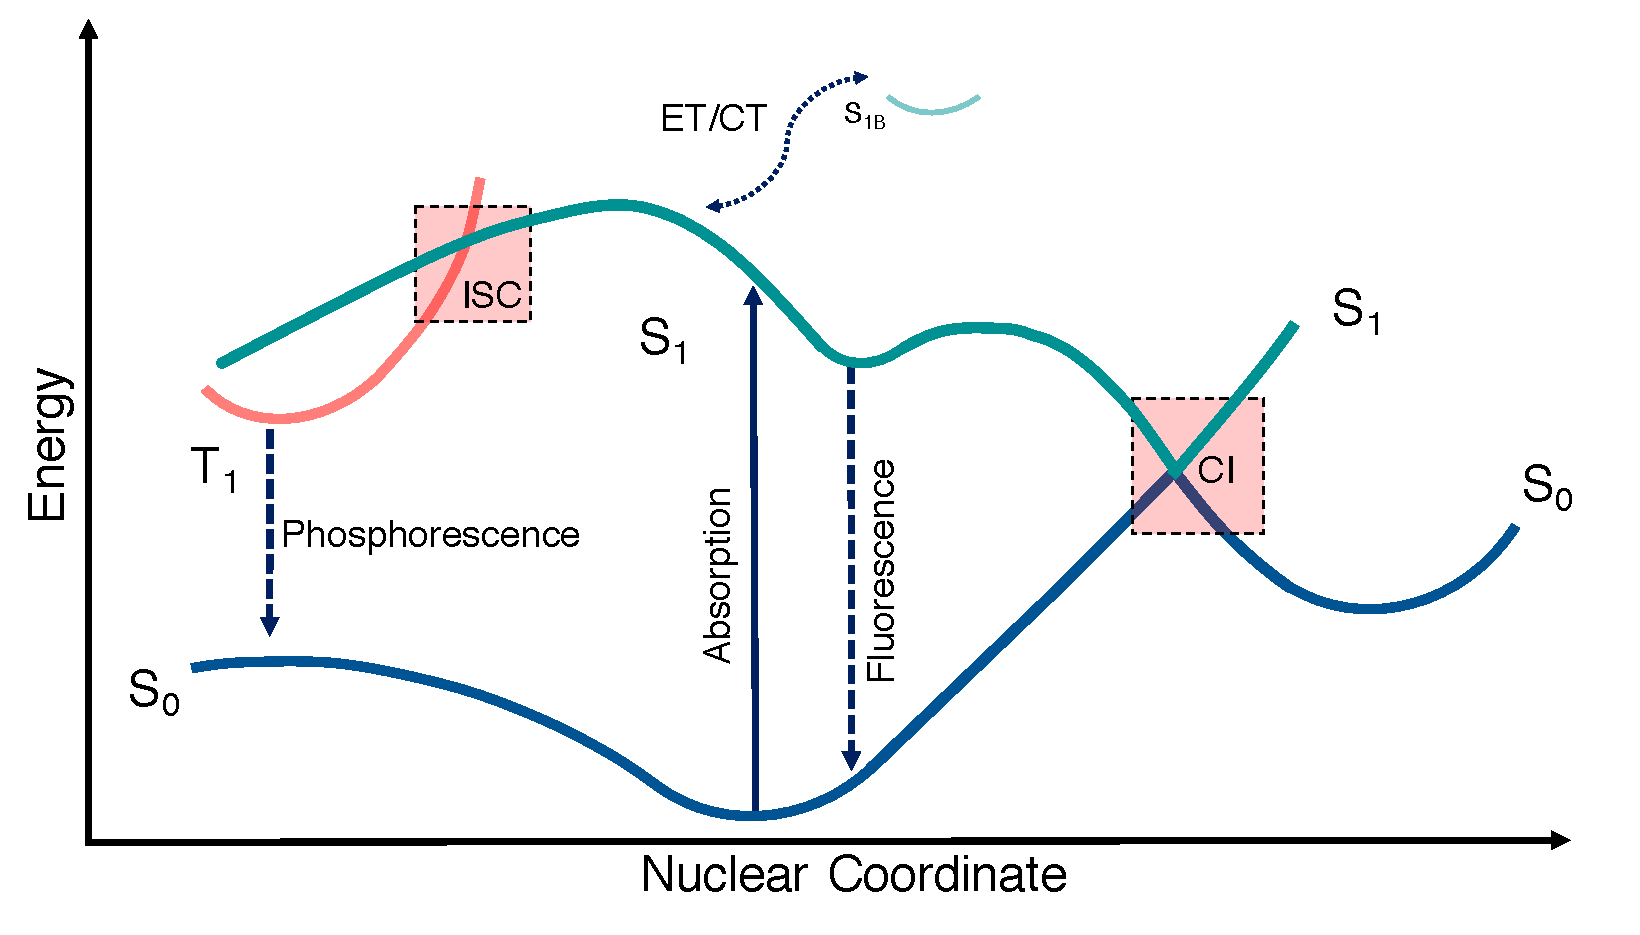
\includegraphics[width=0.8\linewidth]{2Theory/Jablonski.pdf}
  \caption[Relaxation pathways post electronic excitation.]{Competing relaxation pathways after electronic excitation to the first excited singlet state (S\textsubscript{1}. Nonradiative decay channels through conical intersections (CI), energy transfer (ET) and charge transfer (CT) to other molecules, compete with fluorescence. Alternatively, intersystem crossing (ISC) can occur, followed by phosphorescence.}
  \label{figure: Jablonski}
\end{figure}

Electronic excitation, induced by irradiation from the \ac{UV} or visible range, will normally occur at the thermal equilibrium geometry in the ground state. Absorption of a photon will place the system in an electronically excited state. According to the \ac{FC} Principle, the nuclei will undergo negligible change upon change in electronic state. This region of the \ac{PES} is called the \ac{FC} region, or point, and the electronic excitation is considered to be vertical (directly to the point of the upper \ac{PES} vertically above the ground state). From here, a multitude of relaxation processes are possible with vastly different timescales. The fastest process is typically relaxation to lowest vibrational state, occurring in femtoseconds, followed by fluorescence. At the other end of the scale, if there is significant spin-orbit coupling, crossing to a triplet state through \ac{ISC} followed by phosphorescence can take milliseconds. 

Calculating the relative energies of these relaxation pathways is a challenging task for a number of reasons. Firstly, whilst Figure \ref{figure: Jablonski} is a one-dimensional cut of a specific nuclear coordinate, the true \ac{PES} is a 3$N$-6 (3$N$-5 for a linear molecule) hypersurface of nuclear degrees of freedom. As such the full surface cannot feasibly be sampled for large molecules, and specific areas or modes are initally chosen. Secondly, the same ground state methods introduced in Section \ref{section: methods} must be tweaked or expanded upon to incorporate excited states. Thirdly, and perhaps most importantly, in certain regions of the \ac{PES} the fundamental principle of quantum chemical methods, the Born-Oppenheimer approximation, breaks down altogether. Such regions occur when two electronic states become close in energy, as highlighted in red in Figure \ref{figure: Jablonski}. In this region, the electronic states become directly coupled with the nuclear motion, breaking the Born-Oppenheimer approximation. These ``funnel" regions, or conical intersections, are crucial in modelling nonradiatve decay.

This section is organised as follows. Firstly, the importance of conical intersection will be discussed. Following, we will examine how excited-state mechanisms can be probed through nonadiabatic dynamics simulations. Finally, methods to perform these calculations, such as \acf{TDDFT}, shall be addressed. 
\subsection{Conical Intersections} \label{section: photo_conicals}
In photochemical processes with well-defined, well-separated electronic states, the adiabatic Born-Oppenheimer approximation is valid (Equation \ref{equation: BO}). That is, the nuclear wavefunction of an electronic state independent from the nuclear wavefunction of another state. However, as shown in Figure \ref{figure: Jablonski}, in photochemical processes there are regions on the energy landscape where electronic states become close in energy. In these regions, small changes in nuclear configuration results in large changes in the electronic wavefunction - hence the separation of nuclear and electronic wavefunctions is no longer valid and the Born-Oppenheimer approximation breaks down. In practice, this means that the nonadiabtic coupling terms become important and can no longer be neglected. The coupling operator $\hat{\Lambda}$ of Equation \ref{equation: nucwavefunctions} is defined as
\begin{equation}
    \hat{\Lambda}_{IJ}=\frac{1}{2M}(2\bm{F}_{JI}\cdot{}\nabla{}+G_{JI})
\end{equation}
where $\nabla$ the first derivative of position and
\begin{equation}
    \bm{F}_{JI}=\bra{\Phi_{I}}\nabla{}\ket{\Phi_{J}}
\end{equation}
is the derivative or nonadiabatic coupling vector with respect to position. $G_{JI}$ is the scalar coupling,
\begin{equation}
    G_{JI}=\bra{\Phi_{I}}\nabla{}^{2}\ket{\Phi_{J}}.
\end{equation}
$\bm{F}_{JI}$ is a 3$N$-vector coupling the nuclear motion of electronic state $I$ with state $J$. The total value is given by the scalar product of $\bm{F}$ with the nuclear momentum, and so the size (and thus the probability of a transition) is defined by the size of the coupling as well as the momentum of the nuclei.\cite{Worth2004}. The derivative coupling $\bm{F}_{JI}$ can be expressed in terms of the electronic Hamiltonian $H_{e}$, such that
\begin{equation}\label{equation: NAC_F}
        \bm{F}_{JI}=\frac{\bra{\Phi_{I}}\nabla{}\hat{H}_{e}\ket{\Phi_{J}}}{E_{J}-E_{I}}.
\end{equation}

With large electronic differences ($E_{J}-E_{I}$), the large mass difference between electrons and nuclei make $\bm{F}_{JI}$ inconsequentially small. However, as states converge the coupling increases. Only two coordinates can lift complete degeneracy, resulting in the \ac{PES} forming a double-cone structure. Conical intersections thus act as funnels, where the wavepacket can transfer nonradiatively between electronic states in an ultrafast timeframe. The two degrees of freedom define the branching space vectors. The first is the gradient difference vector $\bm{g}$, defining the difference between the gradients of the upper and lower \acp{PES},
\begin{equation}
    \bm{g}_{JI}=\bra{\Phi_{I}}\nabla{}\hat{H}_{e}\ket{\Phi_{I}}-\bra{\Phi_{J}}\nabla{}\hat{H}_{e}\ket{\Phi_{J}}.
\end{equation}
The second is the nonadiabatic coupling vector $\bm{h}$, defining the direction of strongest coupling between states, which is the numerator of Equation \ref{equation: NAC_F},
\begin{equation}
    \bm{h}_{JI}=\bra{\Phi_{I}}\nabla{}\hat{H}_{e}\ket{\Phi_{J}}.
\end{equation}
The vectors $\bm{g}$ and $\bm{h}$ are orthogonal, defining the plane of the conical intersection. $\bm{g}$ points in the direction of removing the energetic splitting, whilst $\bm{h}$ points towards maximising the nonadiabatic coupling. This is depicted in Figure \ref{figure: Cone}. Important to note is that for polyatomic molecules the conical intersection is not an isolated point but multidimensional. Displacement through any of remaining 3$N$-8 coordinates will retain the degeneracy, with the system moving on a degeneracy seam between the two surfaces.
\begin{figure}[H]
\centering
  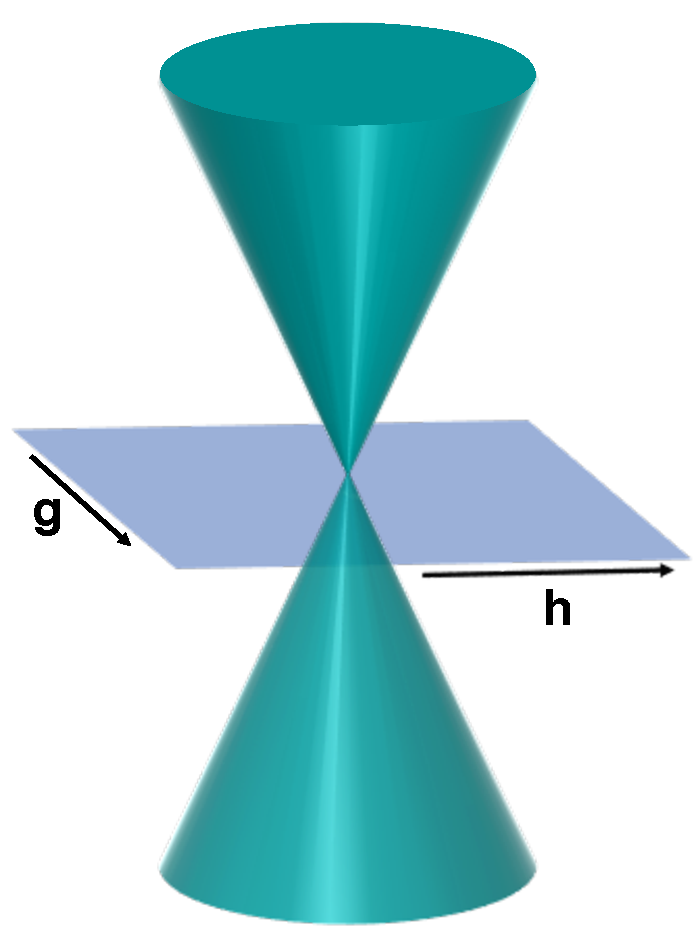
\includegraphics[width=0.4\linewidth]{2Theory/cone.pdf}
  \caption[Schematic of the double-cone topology of degenerate electronic states]{Schematic of the double-cone topology of degenerate electronic states. The gradient difference vector $\bm{g}$ and the nonadiabatic coupling vector $\bm{h}$ define the branching space lifting the degeneracy.}
  \label{figure: Cone}
\end{figure}
Locating conical intersections is important in determining the feasibility of nonradiative decay mechanisms.\cite{Domcke2011} In particular, the \ac{MECI} between the ground and first excited state is a local minimum on the S\textsubscript{1}/S\textsubscript{0} intersection seam and represents the lower bound for feasible crossings. Various methods to locate the geometry of \acp{MECI} for molecular systems have been developed using the gradient difference and nonadiabatic couplings vectors.\cite{Koga1985,Manaa1993,Bearpark1994,Dallos2004,Yarkony2004} 

In the majority of this work, we use the CIOpt algoirthm of Levine, Coe, and Martinez to locate \acp{MECI} for single-reference methods, where the derivative coupling vectors are not required.\cite{Levine2008} In CIOpt, Legrange multipliers are used to find the minimum of the objective function
\begin{equation}\label{equation: CIOpt}
F_{JI}(\bm{R},\sigma{},\alpha{})=\bm{E}_{JI}(\bm{R})+\sigma{}G_{JI}(\Delta{}E_{JI}(\bm{R},\alpha))
\end{equation}
where 
\begin{equation}
    \bm{E}_{JI}(\bm{R})=\frac{E_{I}(\bm{R})+E_{J}(\bm{R})}{2}
\end{equation}
and
\begin{equation}
    \Delta{}E_{JI}(\bm{R})=E_{J}(\bm{R})-E_{I}(\bm{R})
\end{equation}
where $G_{JI}(\Delta{}E_{JI}(\bm{R},\alpha)$ is a penalty function. Equation \ref{equation: CIOpt} minimises the average energy of states $I$ and $J$ with the penalty function penalising any step which increases the energy gap.  $\sigma$ alters the penalty weight whilst $\alpha$ is a smoothing factor. The interfacing of CIOpt with a variety of electronic structure codes allows \acp{MECI} to be located for a variety of quantum chemical methods. 

The topology of conical intersections calculated by different quantum chemical methods has attracted debate in the community.\cite{Levine2006a,Gozem2014,Tuna2015,Lefrancois2017} It has been shown that CASSCF and MS-CASPT2 (but not CASPT2) wavefunctions show the correct double-cone topology and a ``true" conical intersection. However, surfaces obtained with \ac{TDDFT} instead have a linear crossing due to there being no nonadiabatic coupling vector.\cite{Gozem2014}. ADC(2) methods also show a linear intersection, whereas \ac{CC}2 surfaces have the correct conical characteristics but are not completely quantitative.\cite{Tuna2015}. Therefore multireference methods are certainly preferable for modelling S\textsubscript{1}/S\textsubscript{0} crossings. However, single-reference methods can provide a qualitative description of the crossings and can produce reliable geometries. Dynamics simulations with these methods have shown for multiple systems that ADC2 and CC2 can provide reasonable results.\cite{Gozem2014,Tuna2015} In the case of TDDFT, a careful selection of the functional is required.\cite{Crespo-Otero2014,Barbatti2015} With the computational cost of multireference methods and the sensitivity of their active space, in this work we use a combination of single- and multireference methods, where \acp{MECI} obtained with \ac{TDDFT}, \ac{ADC2}, and \ac{CC}2 methods are compared to those obtained with CASSCF.

\subsection{Dynamics Simulations of Excited State Processes}\label{section: photo_dynamics}
Simulation of the temporal evolution of photoinduced processes is a powerful method for probing excited state \acp{PES}. Treating both nuclear and electronic motion fully quantum mechanically, with the required nonadiabatic couplings, is unfeasibly expensive for real molecular systems. As with all quantum chemical approaches, approximations are made. To retain the quantum description of the nuclei, specific nuclear modes can be sampled to reduce the dimensionality of the configuration space and the associated computational cost. Alternatively, the nuclear motion can be treated classically and allowed to explore the configuration space determined by the electronic \acp{PES}. 

The second approach, \ac{NA-MQC}, shall be used in elements of this thesis with the \ac{TSH} method. The most prominent \ac{NA-MQC} methods are \ac{TSH}, mean-field Ehrenfest, and multiple spawning.\cite{Crespo-Otero2018} In Ehrenfest dynamics, a nuclear trajectory is calculated using a weighted-average of a predefined number of electronic states. In multiple spawning, a series of Gaussian functions describe the nuclear wavepacket propagating on electronic surfaces. In the vicinity of state crossings, more Gaussian functions are spawned to follow each electronic state. With \ac{TSH}, a set of independent trajectories approximate the wavepacket propagation, with electronic transitions determined stochastically, most commonly using Tully's fewest-switches alogrithm.\cite{Tully1990} \ac{TSH} is perhaps the mostly used algorithm for simulating \ac{NA-MQC} dynamics, where the Newtonian progpoation of the nuclei, on-the-fly quantum chemical calculations, and straightforward parallelisation have encouraged wide adoption.\cite{Barbatti2011}

In \ac{TSH}, the nuclei propagate classically on a single, adiabatic electronic surface, governed by 
\begin{equation}\label{equation: nuclei_prop}
    \frac{\mathrm{d}^{2}\bm{R}}{\mathrm{d}t^{2}}=\frac{\bm{F}}{M}
\end{equation}
where the force $\bm{F}$ is proportional to the electronic gradient of the current state $I$
\begin{equation}
    \bm{F}=-\nabla{}\bra{\Phi_{I}}\hat{H}_{e}\ket{\Phi_{I}}.
\end{equation}
The nuclear motion is integrated typically using the velocity Verlet algorithm.\cite{Swope1982} At each nuclear timestep, the evolution of the electrons is governed by the time-dependent \schro{} equation, where the wavefunction is approximated as a linear combination of $K$ electronic states $\psi$
\begin{equation}
    \Phi{}=\sum_{K}c_{K}\psi_{K},
\end{equation}
allowing the \schro{} equation to propagate through the coefficients $c$
\begin{equation}\label{equation: sc-schro}
    \frac{\mathrm{d}c_{I}}{\mathrm{d}t}=\sum_{K}-c_{K}\big(\frac{i}{\hbar}H_{IK}+\Lambda_{IK}\big)
\end{equation}
where $H$ collects the energies and $\Lambda$ the nonadiabatic couplings. The time-derivatives of the nonadiabatic couplings can be computed through wavefunction overlaps from previous time steps, using a finite differences procedure.\cite{Pittner2009,Ryabinkin2015}

In practice, the initial state (at $t=0$) is chosen based upon the oscillator strenghts for the nuclear configuration in question. During propagation, the current state can change, or 'hop', from $I$ to $J$ based upon a probability $P$ defined by
\begin{equation}\label{equation: hopping_prob}
    P_{I\rightarrow{}J}=\mathrm{max}\bigg[0,\frac{-2\Delta{}t}{|c_{I}|^{2}}\mathrm{Re}(\Lambda_{IJ}c_{J}c_{I}^{\ast}))\bigg]
\end{equation}
which gives a hopping probability number $P$. For the hop $I\rightarrow{}J$ to occur, a randomly sampled number $r_{t}([0,1])$ is used to evaluate
\begin{equation}\label{equation: hop_condition}
    \sum_{K=1}^{J-1}P_{I\rightarrow{}K}<r_{t}\leq{}\sum_{K=1}^{J}P_{I\rightarrow{}J}
\end{equation}
A further condition that the energy does not increase after a hopping is also enforced. The nuclear equations are typically integrated in steps of \si{0.5}{fs}, while the electronic structure calculated are performed at these timesteps with interpolation between them to account for the faster oscillations to reduce the computational expense. Generally, the algorithm for \ac{TSH} involves the following steps:
\begin{enumerate}
    \item Calculate electronic energies, gradients and nonadiabatic coupling terms for a specific nuclear configuration
    \item Integrate Equation \ref{equation: sc-schro}
    \item Evaluate the hopping probability from Equation \ref{equation: hopping_prob} and determine the current state from Equation \ref{equation: hop_condition}
    \item Propogate the nuclei to a new configuration by integrating Equation \ref{equation: nuclei_prop}
\end{enumerate}
These steps are repeated until the maximum time for the simulation is reached. An ensemble of trajectories is done, where the above alogrithm is carried out for many starting nuclear configurations to obtain the average wavepacket propagation. The most compuationally demanding step is the first, where the electronic properties are calculated at each time step. 

The number of trajectories in the ensemble is important for proper evaluation of the configuration space. However, even with an infinite ensemble, the quantum features of the nuclear motion are generally missed in \ac{TSH}. This is due to the decoherence problem, where forcing the propagation along a single surface artificially prevents the amplitudes following other gradients. By applying a dechorence correction in Step 2., the \ac{TSH} average population of the independent trajectories should mimic the quantum behaviour if enough trajectories are sampled.\cite{Granucci2007} Further corrections in \ac{TSH} must be made in order to preserve kinetic energies in case of frustrated hopping events, where Equation \ref{equation: hopping_prob} is fulfilled but the energy condition is not.

\subsection{Methods for Excited States}\label{section: photo_methods}
One of the most popular methods for probing excited states is \acf{TDDFT}, first proposed in 1984 by Runge and Gross, and then extended in 1995 by Casida, TDDFT is a popular approach for modelling the properties of electronically excited states[66]. The fundamental idea within TDDFT is that the dynamics of a system can be completely described by its time-dependent density. Runge and Gross proved that there is a unique, 1:1 correspondence between time-dependent densities and potentials.\cite{Runge1984}  From the 1:1 correspondence it follows that the time-dependent density is a unique functional of the external potential (and vice versa). The time-dependent Hamiltonian, and thus the wavefunction, are also functionals of the density, allowing the deduction that all physical observables are functionals of the time-dependent density.

The key quantity in determining the time-dependent density in \ac{TDDFT} is the time-dependent \acf{XC} energy. Just as in \ac{DFT}, \ac{TDDFT} requires a suitable approximation of the \ac{XC}-energy. \ac{TDDFT} uses the \ac{XC}-energy from \ac{DFT} and to construct the time-dependent density, in what is known as the adiabatic approximation. The adiabatic approximation assumes that at each moment in time the \ac{XC}-energy depends only on the instantaneous density. Excitations are calculated in \ac{TDDFT} using linear response theory, which probes the response of a system to a weak perturbation.

A well-known failing in \ac{TDDFT} is the poor description of \acf{CT} excitations, where there is minimal orbital between occupied and virtual orbitals involved in a transition. TDDFT is known to underestimate \ac{CT}-excitation energies with \ac{LDA}, \ac{GGA}, and hybrids, since self-interaction means virtual orbital energies are systematically too low in energy. The \ac{RSH} functionals have been shown to mitigate this error for \ac{CT} excitations, with tuned \ac{RSH} functionals showing equivalent performance wave function methods for the prediction of excitation energies.\cite{Stein2009a,Kuritz2011,Kronik2012a} Within the current work, the \ac{RSH} functional $\omega$B97X-D is used in density functional calculations to incorporate these benefits.\cite{Chai2008} 

In addition, approximate \ac{CC} methods are used to calculate excited state properties of molecules, namely the \ac{CC}2 method. The \ac{CC}2 method was formulated in 1995 to approximate CCSD but with $N^{5}$ scaling and provide accurate excitation energies.\cite{Christiansen1995} In \ac{CC}2, the single excitations of CCSD are retained but the double excitations are approximated, with comparable ground state accuracy of MP2.\cite{Hattig2005} Response functions of \ac{CC}2 provide excitation energies and transition moments, making it a popular method in probing excited-state properties of molecules.\cite{Sneskov2012}

As an alternative but closely related approach, propagator methods are also used to calculate excitation energies and transition moments. The polarizer propagator introduces the effect of an external field, for instance the absorption of a photon. In the \ac{ADC2}, the polarizer propagator acts on the \ac{MP2} ground state to give excitation energies at similar accuracy but reduced computational cost compared to \ac{CC}2.

\subsection{Modelling Excited States in Molecular Crystals} \label{section: excited_states_crystals}
The theoretical treatment of excitations in molecular crystals is a relatively underdeveloped field compared to modelling of excited states in solution or even band gaps in periodic solids. The localised nature of excited states in molecular crystals lends to a molecular orbital description, since the excited state resides on typically one or two molecular units.\cite{Sauer1989} The low population of excited molecules in the crystal has led to the current practice of modelling clusters of molecules extracted from the crystal structure. In this methodology, the cluster is partitioned into regions which are treated at different levels of theory in ``multilayer" models. At the centre of a cluster lies a chromophore molecules (or molecules), to be treated at an appropriate level using quantum mechanical methods. To reduce the computational expense, the contribution of the surrounding environmental molecules to the total energy is calculated a lower level of theory, either through a \acf{MM} description (denoted QM:MM) or an efficient quantum mechanical method such as \ac{HF} (QM:QM'). QM:QM' approaches combining multireference methods with DFT are a promising extension, although the they have not yet been widely used in describing excited state phenomena.\cite{Libisch2014,Cheng2017,Cheng2017a} It is typical to freeze the positions of the environmental atoms to retain the crystal packing arrangement, such that only the QM atoms are allowed to relax during an optimisation. It is therefore desirable to first optimise the unit cell using plane wave methods.\cite{Presti2016} 

A popular route to obtaining the total energy of the cluster is the ONIOM method.\cite{Byun1999,Frisch2003,Chung2015a} In the field of \ac{AIE}, the multilayer ONIOM QM:MM protocol has been applied in many studies to understand the fluorescent behaviour of solid state organic compounds.\cite{Li2011,Li2013,Sun2015a,Presti2016a,Wilbraham2016,Wang2016,Peng2016,Fan2016,Presti2017a,Li2017b,Lin2017,Li2017e,Fan2017,Hestand2017} In the ONIOM method, the whole cluster is called the ``real" system and the region to be treated at the highest level of theory is laballed as the ``model". The total energy ($E_{ONIOM}$) for the cluster is calculated through a subtractive scheme,
\begin{equation}\label{equation: ONIOM}
E_{ONIOM}=E_{QM,Model}+E_{MM,real}-E_{MM,model}
\end{equation}
where the total energy is the sum of the QM energy of the model system with the MM energy of the real system. Subtracting the energy of the model system at the MM level ensures that its contribution is not double counted.\cite{Chung2015a} The QM level energy is calculated through the chosen method, typically (TD)DFT or CASSCF/CASPT2. The MM-level energy is obtained, for the Amber forcefield, through

\begin{equation}
\begin{split}
    E_{MM}&=\sum_{bonds}K_{r}(r-r_{eq})^{2}+\sum_{angles}K_{\theta}(\theta-\theta_{eq})^{2}+\sum_{dihedrals}\frac{V_{n}}{2}[1+\mathrm{cos}(n\phi{}-\gamma{})]\\
    &+\sum_{i<j}\bigg[s_{ij}^{VdW}\big(\frac{A_{ij}}{r_{ij}^{12}}-\frac{B_{ij}}{r_{ij}^{6}}\big)+s^{q}_{ij}\frac{q_{i}q_{j}}{\epsilon{}r_{ij}}\bigg].
\end{split}
\end{equation}
The first three terms evaluate the bonded interactions through chemical bonds, angles and dihedrals. The final non-bonded interaction term describes the van der Waals and Coulomb interaction between each atom in the system, which are scaled by $s^{vdW}$ and $s^{q}$.
In mechanical embedding, the cross-region electrostatic interactions are treated at the MM level, and as such the electronic Hamiltonian is not polarised (or influenced) by the environmental molecules. In electrostatic embedding, atom-centred point charges from the MM region are incorporated into the QM Hamiltonian $\hat{H}_{V}^{model,QM}$ by modifying the original Hamiltonian $\hat{H}^{model,QM}$
\begin{equation}
    \hat{H}_{V}^{model,QM}=\hat{H}^{model,QM}-\sum_{i}\sum_{N}\frac{s_{N}q_{N}}{r_{iN}}+\sum_{J}\sum_{N}\frac{Z_{J}s_{N}q_{N}}{r_{JN}}
\end{equation}
where $N$,$J$, and $i$ refer to the MM atoms, QM atoms, and electrons respectively.\cite{Vreven2006} The scaling factor $s_{N}$ prevents overpolarisation of the wavefunction from atoms close to the QM region. The final term is also included in the MM evaluation of the model system, to ensure direct cancellation. The electrostatic embedding scheme provides a direct perturbation of the electronic structure by the environment. 

A potential deficiency arising from a standard ONIOM calculation for a cluster model is the neglect of the periodic nature of the molecular crystal. The truncation of the crystal into a cluster naturally removes the electrostatic long-range potential. To overcome this, other fields have research have applied the Ewald summation technique, which calculates the exact nature of the crystalline electrostatic potential.\cite{Weber2010,Stueber2001b} The Ewald method as implemented by Derenzo and coworkers does this through a five step algorithm:\cite{Klintenberg2000,Derenzo2000}  
\begin{enumerate}
    \item the point charges from a unit cell are assigned to the atoms of a supercell centered around a defect of interest called the quantum cluster.
    \item A chosen number of sample sites are randomly sampled in the quantum cluster region.
    \item A spherical region is then defined so that the quantum cluster and a number of additional points are included within a chosen radius. The points within that region will maintain their original charge values whereas the remaining points will be allowed to vary.
    \item An Ewald potential is calculated at each fixed value point (including points in the quantum cluster) and at the random sites from step 2.
    \item A system of linear equations is solved with respect to the variable charge values to match the direct sum of all charges in the system to the Ewald potentials calculated in step 4, whilst driving the overall charge and dipole moment to zero.
\end{enumerate}
The Ewald method was applied to excited states in molecular crystals in 2016 by Wilbraham \textit{et al.}\cite{Wilbraham2016} As the authors point out, the Ewald scheme is superior to traditional point charge embedding which inevitably involves some kind of charge truncation and the subsequent loss of periodicity. The Ewald method in contrast aims to reproduce the exact potential on the chromophore. For their case, an ESIPT/AIE system was chosen as a test molecule, such is the importance of the environment on the electronic structure. 
A second shortcoming of the ONIOM approach alone for excited states is the lack of polarisation of the MM region from the QM region. In the electrostatic embedding scheme, the QM region is polirased by the MM environment, but there is no mutual polarisation from the QM region \textit{back} to the MM atoms. Wilbraham and co-workers have attempted to remedy this through a self-consistent polarisation scheme, where the MM point charges and QM charges are altered until convergence.\cite{Wilbraham2016} This has been shown to be more effective than embedding alone for modelling absorption and emission in molecular crytals.\cite{Presti2017a,Wilbraham2018a} However, by treating the environment point charges and the chromophore charges at the same level of theory, the former necessarily correspond to a fully excited molecular crystal, which is perhaps nonphysical. This has been addressed by Miguel Rivera in our group, who has worked on the development of self-consistent embedding schemes to extend the method of Wilbraham. There are implemented in the \texttt{fromage} package. Due to the implementation timeline, self-consistent embedding schemes were not included in the work of this thesis. 
